% \documentclass[handout]{beamer} % TEMP: handout collapses overlays for faster builds; remove [handout] to restore
\documentclass{beamer}

\usepackage{mpemath}
\usepackage{subcaption}
\usepackage[normalem]{ulem}
\usepackage{amsmath}
\usepackage{amssymb}
\usepackage{mathtools}
\usepackage{booktabs}
\usepackage{siunitx}
\usepackage{natbib}
\usepackage{tabularx}
\usepackage{multirow}
\usepackage{bbm}
\usepackage[dvipsnames]{xcolor} % Saved my life during a conference once
\usepackage{tikz}
\usetikzlibrary{arrows.meta,positioning,matrix,calc,fit,backgrounds}
\usepackage{listings}

% *** Styles ***
\usetheme{Singapore}
\setbeamertemplate{navigation symbols}{}
\setbeamercovered{invisible}
\usefonttheme{professionalfonts}
\setbeamertemplate{footline}[frame number]

% *** Code listings ***
\lstdefinestyle{py}{
  language=Python,
  basicstyle=\ttfamily\scriptsize,
  keywordstyle=\color{NavyBlue}\bfseries,
  commentstyle=\color{Gray}\itshape,
  stringstyle=\color{BrickRed},
  showstringspaces=false,
  breaklines=true,
  frame=single,
  rulecolor=\color{lightgray},
  columns=fullflexible,
  keepspaces=true,
}
\lstset{style=py}

% *** Running example ***
\colorlet{itcolor}{BrickRed}
\colorlet{catcolor}{NavyBlue}
\colorlet{fishcolor}{ForestGreen}
\colorlet{adjcolor}{Plum}
\newcommand{\sentstem}{The \textcolor{adjcolor}{fluffy} \textcolor{catcolor}{cat} eats \textcolor{adjcolor}{fresh} \textcolor{fishcolor}{fish} because \textcolor{itcolor}{it} is}
\newcommand{\srcsent}{\sentstem{} hungry.}
\newcommand{\altsent}{\sentstem{} tasty.}
\newcommand{\blanksent}{\sentstem{} \underline{\hspace{2em}}}
\newcommand{\tok}[2][gray]{\tikz[baseline=(t.base)]\node[draw=#1,rounded corners=2pt,inner sep=2pt,fill=#1!10](t){\strut\texttt{#2}};}
\newcommand{\sentoks}{{\footnotesize \tok{The} \tok[adjcolor]{fluffy} \tok[catcolor]{cat} \tok{eats} \tok[adjcolor]{fresh} \tok[fishcolor]{fish} \tok{because} \tok[itcolor]{it} \tok{is} \tok{hungry}}}
\newcommand{\shape}[1]{\texttt{(#1)}}
\newcommand{\mquery}{\textbf{\textcolor{itcolor}{Query}}}
\newcommand{\mkey}{\textbf{\textcolor{catcolor}{Key}}}
\newcommand{\mvalue}{\textbf{\textcolor{fishcolor}{Value}}}
\colorlet{qcolor}{itcolor}
\colorlet{kcolor}{catcolor}
\colorlet{vcolor}{fishcolor}
\newcommand{\vq}{\mathcolor{qcolor}{\bm{q}}}
\newcommand{\vk}{\mathcolor{kcolor}{\bm{k}}}
\newcommand{\vv}{\mathcolor{vcolor}{\bm{v}}}
\newcommand{\mQ}{\mathcolor{qcolor}{\bm{Q}}}
\newcommand{\mK}{\mathcolor{kcolor}{\bm{K}}}
\newcommand{\mV}{\mathcolor{vcolor}{\bm{V}}}
\newcommand{\WQ}{\mathcolor{qcolor}{\bm{W}}^{\mathcolor{qcolor}{\bm{Q}}}}
\newcommand{\WK}{\mathcolor{kcolor}{\bm{W}}^{\mathcolor{kcolor}{\bm{K}}}}
\newcommand{\WV}{\mathcolor{vcolor}{\bm{W}}^{\mathcolor{vcolor}{\bm{V}}}}

\newcommand{\cc}[1]{\textcolor{red}{[CC: #1]}} % review comments
% token box inside a tikzpicture (\tok is itself a tikz node)
\tikzset{
  atok/.style={draw=#1, fill=#1!10, rounded corners=2pt, inner sep=2pt, text height=1.6ex, text depth=0.4ex, font=\ttfamily\footnotesize},
  atok/.default=gray,
}
% \sentnodes{p} inside a tikzpicture places the sentence as nodes p0 ... p9
\newcommand{\sentnodes}[2][]{%
  \node[atok] (#20) {The};
  \node[atok=adjcolor, right=2pt of #20] (#21) {fluffy};
  \node[atok=catcolor, right=2pt of #21] (#22) {cat};
  \node[atok, right=2pt of #22] (#23) {eats};
  \node[atok=adjcolor, right=2pt of #23] (#24) {fresh};
  \node[atok=fishcolor, right=2pt of #24] (#25) {fish};
  \node[atok, right=2pt of #25] (#26) {because};
  \node[atok=itcolor, right=2pt of #26] (#27) {it};
  \node[atok, right=2pt of #27] (#28) {is};
  \node[atok, right=2pt of #28, #1] (#29) {hungry};
}

\title{Transformers}
\author{Gersi Doko}
\institute{Department of Computer Science \\ University of New Hampshire}
\date{}

\AtBeginSection[]{
  \begin{frame}
    \vfill
    \centering
    % \usebeamerfont{title}
    {\huge\bf \insertsection}%
    \vfill
  \end{frame}
}

\begin{document}

\frame{\titlepage}

\section*{Intro}

\begin{frame}
  \frametitle{Language is Annoying}
  \vfill
  \centering
  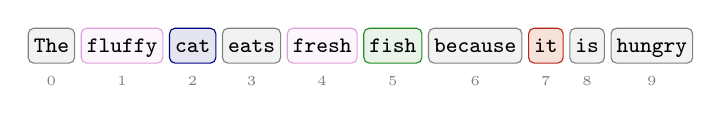
\begin{tikzpicture}
    \sentnodes{op}
    \foreach \i in {0,...,9} {
      \node[font=\tiny, text=gray, below=1pt of op\i] {\i};
    }
  \end{tikzpicture}
  \vfill
\end{frame}

\begin{frame}
  \frametitle{Words Depend on Each Other}
  \vfill
  \centering
  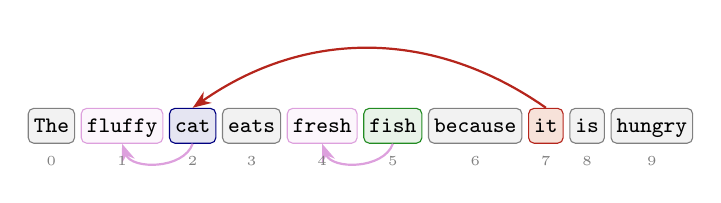
\begin{tikzpicture}
    \sentnodes{oc}
    \draw[-{Stealth}, adjcolor, thick] (oc2.south) to[bend left=70] (oc1.south);
    \draw[-{Stealth}, adjcolor, thick] (oc5.south) to[bend left=70] (oc4.south);
    \draw<3->[-{Stealth}, itcolor, thick] (oc7.north) to[bend right=35] (oc2.north);
    % reserve the space of the it -> cat arc on every overlay
    \path (oc2.north) ++(0, 0.9);
    \foreach \i in {0,...,9} {
      \node[font=\tiny, text=gray, below=1pt of oc\i] {\i};
    }
  \end{tikzpicture}
  \vfill
\end{frame}

\begin{frame}
  \frametitle{Making a Key Assumption}
  \vfill
  \centering
  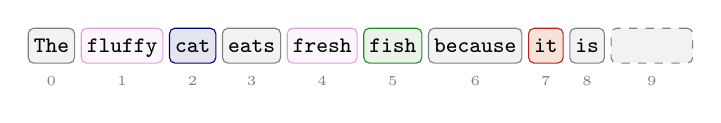
\begin{tikzpicture}
    \sentnodes[dashed, text opacity=0]{ob}
    \foreach \i in {0,...,9} {
      \node[font=\tiny, text=gray, below=1pt of ob\i] {\i};
    }
  \end{tikzpicture}
  \vfill
  \centering
  \emph{hungry} $\Rightarrow$ \tok[itcolor]{it} =
  \tok[catcolor]{cat}, \emph{tasty} $\Rightarrow$
  \tok[itcolor]{it} = \tok[fishcolor]{fish}
  \vfill
\end{frame}

\begin{frame}
  \frametitle{Natural Questions}
  \vfill
  \begin{enumerate}[Q1]
    \item<1-> What is a word, to a computer?
    \item<1-> Does order matter? - ``The fresh fish eats fluffy cat''?
    \item<1-> What does \textcolor{itcolor}{it} refer to?
    \item<1-> What is the \textcolor{catcolor}{cat} like?
    \item<1-> Can one word take on multiple meanings?
  \end{enumerate}
  \vfill
\end{frame}

% Decoder-only architecture, the visual backbone of the talk.
% Shown with <1> here; later sections revisit it with \againframe<k>{decarch}:
% <1> empty "?" box, <2> + Embed, Pos. Enc. greyed out (Q1), <3> + Pos. Enc. (Q2),
% <4> + Norm -> Masked Multi-Head Self-Attention -> (+) (Q3-Q6),
% <5> + Norm -> Feed Forward -> (+), block xN, final Norm (Q7, Q8),
% <6> + Linear + log_softmax (Q9)
\begin{frame}<1>[label=decarch]
  \frametitle{Decoder-Only Architecture}
  \centering
  \makebox[\textwidth][c]{%
    \begin{tikzpicture}[
        x=1cm, y=1.2cm, font=\footnotesize,
        >={Stealth[length=3pt]},
        dablk/.style={draw, rounded corners=2pt, minimum width=2.9cm,
        minimum height=0.42cm, inner sep=1pt, align=center},
        daattn/.style={dablk, fill=orange!25, minimum height=0.72cm},
        daffn/.style={dablk, fill=cyan!15},
        danorm/.style={dablk, fill=yellow!35},
        daemb/.style={dablk, fill=red!12},
        dagen/.style={dablk, fill=violet!15},
        daadd/.style={draw, circle, fill=white, inner sep=0pt,
        minimum size=0.34cm, font=\footnotesize},
        dacls/.style={font=\scriptsize\ttfamily, text=black!75, inner sep=1pt,
        anchor=east, align=right},
        daq/.style={font=\footnotesize, inner sep=1pt, anchor=west, align=left},
        daio/.style={font=\footnotesize, inner sep=1pt},
        daunk/.style={draw=gray, dashed, thick, rounded corners=4pt, fill=gray!6},
      ]
      % ---------- input and output (every stage) ----------
      \node[daio] (dain) at (0, 0)
      {\texttt{<s> The fluffy \dots\ it is} \shape{1, 10}};
      \node[daio] (daout) at (0, 5.3) {next-token log-probs \shape{1, 10, V}};
      \draw[->] (dain.north) -- (0, 0.37);
      \draw[->] (0, 4.93) -- (daout.south);
      % ---------- not yet discovered: dashed "?" box ----------
      \only<1>{
        \draw[daunk] (-2.05, 0.37) rectangle (2.05, 4.93);
        \node[font=\Huge, text=gray] at (0, 2.65) {?};
      }
      \only<2-3>{
        \draw[daunk] (-2.05, 0.88) rectangle (2.05, 4.93);
        \node[font=\Huge, text=gray] at (0, 2.9) {?};
      }
      \only<4>{
        \draw[daunk] (-2.05, 2.52) rectangle (2.05, 4.93);
        \node[font=\Huge, text=gray] at (0, 3.72) {?};
      }
      \only<5>{
        \draw[daunk] (-1.45, 4.57) rectangle (1.45, 4.93);
        \node[font=\footnotesize, text=gray] at (0, 4.75) {?};
      }
      % ---------- <2> embeddings + positional encoding ----------
      \only<2->{
        \node[daemb] (daemb) at (0, 0.55) {Embed \textcolor<2>{black!30}{+ Pos.\ Enc.}};
      }
      \only<2-3>{\draw[->] (daemb.north) -- (0, 0.88);}
      % ---------- <4> masked self-attention sublayer ----------
      \only<4->{
        \node[danorm] (dan1) at (0, 1.1) {LayerNorm};
        \node[daattn] (daatt) at (0, 1.69) {Masked Multi-Head\\Self-Attention};
        \node[daadd] (daad1) at (0, 2.24) {$+$};
        \draw[->] (daemb.north) -- (dan1.south);
        \draw[->] (dan1.north) -- (daatt.south);
        \draw[->] (daatt.north) -- (daad1.south);
        \draw[->, rounded corners=2pt] (0, 0.85) -| (1.6, 2.24) -- (daad1.east);
      }
      \only<4>{\draw[->] (daad1.north) -- (0, 2.52);}
      % ---------- <5> feed-forward sublayer, block xN, final norm ----------
      \only<5->{
        \node[danorm] (dan2) at (0, 2.7) {LayerNorm};
        \node[daffn] (daff) at (0, 3.18) {Feed Forward};
        \node[daadd] (daad2) at (0, 3.62) {$+$};
        \node[danorm] (dafn) at (0, 4.2) {LayerNorm};
        \draw[->] (daad1.north) -- (dan2.south);
        \draw[->] (dan2.north) -- (daff.south);
        \draw[->] (daff.north) -- (daad2.south);
        \draw[->] (daad2.north) -- (dafn.south);
        \draw[->] (dafn.north) -- (0, 4.57);
        \draw[->, rounded corners=2pt] (0, 2.45) -| (1.6, 3.62) -- (daad2.east);
        \draw[rounded corners=4pt, black!60] (-2.05, 0.77) rectangle (2.05, 3.9);
        \node[font=\footnotesize\bfseries, text=black!75] at (-1.75, 2.35) {};
      }
      % ---------- <6> generator ----------
      \only<6->{
        \node[dagen] (dagen) at (0, 4.75) {Linear + log\_softmax};
      }
      % ---------- class names (left) ----------
      \only<2->{
        \node[dacls] at (-2.2, 0.55) {Embeddings\\\textcolor<2>{black!30}{+ PositionalEncoding}};
      }
      \only<4->{
        \node[dacls] at (-2.2, 1.69) {MultiHeadedAttention\\+ subsequent\_mask};
      }
      \only<5->{
        \node[dacls] at (-2.2, 2.45) {ResidualConnection};
        \node[dacls] at (-2.2, 3.18) {PositionwiseFeedForward};
        \node[dacls] at (-2.2, 3.72) {\textbf{EncoderLayer} $\times N$\\};
        \node[dacls] at (-2.2, 4.2) {};
      }
      \only<6->{
        \node[dacls] at (-2.2, 4.75) {Generator};
      }
    \end{tikzpicture}%
  }
\end{frame}

\begin{frame}[fragile]
  \frametitle{The Big Picture}
  % not in transformer.py: forward of the tested DecoderOnlyLM assembly (SCRATCH/decoder_only/assembly_snippet.py)
\begin{lstlisting}
class DecoderOnlyLM(nn.Module):
    ...
    def forward(self, x):
        mask = Batch.subsequent_mask(x.size(1))
        return self.generator(self.blocks(self.embed(x), mask))
\end{lstlisting}
  \vfill
  \begin{enumerate}
    \item<2-> What are the inputs? - \texttt{x} \shape{1, 10}, tokens
    \item<3-> What are the outputs? - next token log-probs \shape{1, 10, V}
    \item<4-> ``\dots because it is'', how likely is \texttt{hungry}? \texttt{tasty}?
    \item<5-> The rest of the talk - what is inside \texttt{embed}, \texttt{blocks}, \texttt{generator}, and why
  \end{enumerate}
  \vfill
\end{frame}

\section*{Words}

\begin{frame}
  \frametitle{Word to Vec - 2013}
  \vfill
  \centering
  {\footnotesize
    \setlength{\tabcolsep}{1pt}
    \begin{tabular}{cccccccccc}
      \tok{The} & \tok[adjcolor]{fluffy} & \tok[catcolor]{cat} & \tok{eats} &
      \tok[adjcolor]{fresh} & \tok[fishcolor]{fish} & \tok{because} &
      \tok[itcolor]{it} & \tok{is} & \tok{hungry} \\
      $\downarrow$ & $\downarrow$ & $\downarrow$ & $\downarrow$ &
      $\downarrow$ & $\downarrow$ & $\downarrow$ & $\downarrow$ &
      $\downarrow$ & $\downarrow$ \\
      \texttt{17} & \texttt{\textcolor{adjcolor}{5120}} &
      \texttt{\textcolor{catcolor}{942}} & \texttt{3051} &
      \texttt{\textcolor{adjcolor}{2764}} &
      \texttt{\textcolor{fishcolor}{1288}} & \texttt{406} &
      \texttt{\textcolor{itcolor}{39}} & \texttt{25} & \texttt{2210} \\
    \end{tabular}
  }
  \vfill
  \raggedright
  \begin{enumerate}
    \item An integer - every token in the vocabulary $V$ gets an id
    \item<2-> \texttt{tokens} = \texttt{[[17, 5120, 942, 3051, 2764, 1288, 406, 39, 25, 2210]]} - shape \shape{1, 10}
    \item<3-> Some token id's are special \texttt{0} = \texttt{<pad>}, \texttt{1} = \texttt{<s>}, \texttt{2} = \texttt{</s>}, \texttt{3} = \texttt{<unk>}, \dots
  \end{enumerate}
  \vfill
\end{frame}

\begin{frame}[fragile]
  \frametitle{Embeddings}
  % transformer.py L75-88
  \vfill
  \begin{lstlisting}
  class Embeddings(nn.Module):
      def __init__(self, d_model, vocab):
          super(Embeddings, self).__init__()
          self.lut = nn.Embedding(vocab, d_model)
          self.scale_term = math.sqrt(d_model)
      def forward(self, x):
          return self.lut(x) * self.scale_term
  \end{lstlisting}
  \vfill
\end{frame}

\begin{frame}
  \frametitle{A (Learnable) Lookup Table}
  \vfill
  \centering
  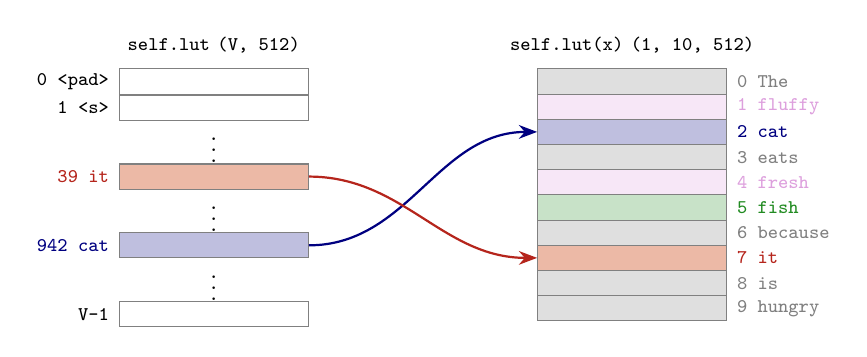
\begin{tikzpicture}[
      embrow/.style={draw=gray, minimum width=2.4cm, minimum height=0.32cm,
      inner sep=0pt, font=\scriptsize\ttfamily},
      emblab/.style={font=\scriptsize\ttfamily, anchor=east},
    ]
    % the table
    \node[embrow] (embr0) {};
    \node[embrow, below=0pt of embr0] (embr1) {};
    \node[embrow, below=0pt of embr1, draw=none] (embrd1) {$\vdots$};
    \node[embrow, below=0pt of embrd1, fill=itcolor!25] (embrit) {};
    \node[embrow, below=0pt of embrit, draw=none] (embrd2) {$\vdots$};
    \node[embrow, below=0pt of embrd2, fill=catcolor!25] (embrcat) {};
    \node[embrow, below=0pt of embrcat, draw=none] (embrd3) {$\vdots$};
    \node[embrow, below=0pt of embrd3] (embrV) {};
    \node[emblab] at (embr0.west) {0 <pad>};
    \node[emblab] at (embr1.west) {1 <s>};
    \node[emblab, text=itcolor] at (embrit.west) {39 it};
    \node[emblab, text=catcolor] at (embrcat.west) {942 cat};
    \node[emblab] at (embrV.west) {V-1};
    \node[font=\scriptsize, above=2pt of embr0] {\texttt{self.lut} \shape{V, 512}};
    % the output
    \foreach \t/\c [count=\i from 0] in {The/gray, fluffy/adjcolor,
      cat/catcolor, eats/gray, fresh/adjcolor, fish/fishcolor,
    because/gray, it/itcolor, is/gray, hungry/gray} {
      \node[embrow, fill=\c!25, anchor=north west]
      (embo\i) at ($(embr0.north east) + (2.9cm, -\i*0.32cm)$) {};
      \node[font=\scriptsize\ttfamily, anchor=west, text=\c] at (embo\i.east) {\i\ \t};
    }
    \node[font=\scriptsize, above=2pt of embo0] {\texttt{self.lut(x)} \shape{1, 10, 512}};
    \draw[-Stealth, catcolor, thick] (embrcat.east) to[out=0, in=180] (embo2.west);
    \draw[-Stealth, itcolor, thick] (embrit.east) to[out=0, in=180] (embo7.west);
  \end{tikzpicture}
  \vfill
  \raggedright
  \begin{enumerate}
    \item<2-> Same id $\Rightarrow$ same row: \tok[itcolor]{it} gets the
      same vector in every sentence - whether it means the cat or the fish
  \end{enumerate}
  \vfill
\end{frame}

\againframe<2>{decarch}

\begin{frame}
  \frametitle{Order}
  \vfill
  \centering
  {\footnotesize
    \tok{The} \tok[adjcolor]{fluffy} \tok[catcolor]{cat} \tok{eats}
    \tok[adjcolor]{fresh} \tok[fishcolor]{fish}
    \vfill
    \tok{The} \tok[adjcolor]{fresh} \tok[fishcolor]{fish} \tok{eats}
    \tok[adjcolor]{fluffy} \tok[catcolor]{cat}
  }
  \vfill
\end{frame}

\begin{frame}
  \frametitle{Positional Encoding}
  \vfill
  \centering
  $PE_{(pos, 2i)} = \sin(pos \cdot \omega_i)$ \qquad
  $PE_{(pos, 2i+1)} = \cos(pos \cdot \omega_i)$ \\[0.3em]
  $\omega_i = 1 / 10000^{2i/d_{model}}$, \quad $i = 0, \dots, 255$
  \vfill
  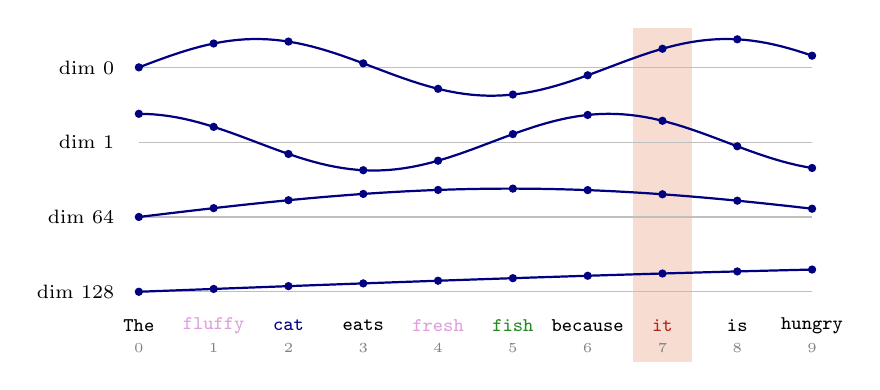
\begin{tikzpicture}[x=0.95cm, y=0.36cm]
    \fill<2->[itcolor!12] (6.6, -10.4) rectangle (7.4, 1.4);
    \foreach \lab/\w/\f [count=\k from 0] in {
    {dim 0}/1/sin, {dim 1}/1/cos, {dim 64}/0.31623/sin, {dim 128}/0.1/sin} {
      \begin{scope}[yshift=-\k*0.95cm]
        \draw[gray!50] (0, 0) -- (9, 0);
        \node[font=\scriptsize, anchor=east] at (-0.2, 0) {\lab};
        \draw[thick, NavyBlue, domain=0:9, samples=90]
        plot (\x, {\f(\w*\x r)});
        \foreach \p in {0, ..., 9} {
          \fill[NavyBlue] (\p, {\f(\w*\p r)}) circle (1.5pt);
        }
      \end{scope}
    }
    \foreach \t/\c [count=\p from 0] in {The/black, fluffy/adjcolor,
      cat/catcolor, eats/black, fresh/adjcolor, fish/fishcolor,
    because/black, it/itcolor, is/black, hungry/black} {
      \node[font=\scriptsize\ttfamily, text=\c] at (\p, -9.1) {\t};
      \node[font=\tiny, gray] at (\p, -9.9) {\p};
    }
  \end{tikzpicture}
  \vfill
  \raggedright
  \begin{enumerate}
    \item<2-> The shaded column (4 of its 512 dims) is added to
      \tok[itcolor]{it} - every position gets its own pattern
    \item<3-> Fast waves tell neighbors apart, slow waves tell far-apart
      positions apart
  \end{enumerate}
\end{frame}

\begin{frame}[fragile]
  \frametitle{Positional Encoding - The Code}
  % transformer.py L96-113
\begin{lstlisting}[basicstyle=\ttfamily\tiny]
class PositionalEncoding(nn.Module):
    def __init__(self, d_model, dropout=0.1, max_len=5000):
        super(PositionalEncoding, self).__init__()
        self.dropout = nn.Dropout(dropout)
        pe = torch.zeros(max_len, d_model)
        position = torch.arange(0, max_len).unsqueeze(1)
        div_term = torch.exp(torch.arange(0, d_model, 2) * -(math.log(10000.0) / d_model))
        pe[:, 0::2] = torch.sin(position * div_term)
        pe[:, 1::2] = torch.cos(position * div_term)
        pe = pe.unsqueeze(0)
        self.register_buffer('pe', pe)
    def forward(self, x):
        x = x + Variable(self.pe[:, :x.size(1)], requires_grad=False)
        return self.dropout(x)
\end{lstlisting}
  \vfill
  {\footnotesize
    \begin{enumerate}
      \item<1-> ``the word \textcolor{itcolor}{\texttt{it}}'' - knows nothing about \textcolor{catcolor}{\texttt{cat}} or \textcolor{fishcolor}{\texttt{fish}}
    \end{enumerate}
  }
  \vfill
\end{frame}

\againframe<3>{decarch}

\section*{Attention}

\begin{frame}
  \frametitle{Who Is \textcolor{itcolor}{\texttt{it}}? Queries, Keys, Values}
  \vfill
  \centering
  \begin{tikzpicture}
    \sentnodes{qa}
    \only<1>{
      \foreach \j in {0,...,6} {
        \draw[-{Stealth}, gray] (qa7.north) to[bend right=35] (qa\j.north);
      }
      \draw[-{Stealth}, gray] ([xshift=2pt]qa7.north) to[out=70, in=110, looseness=12] ([xshift=-2pt]qa7.north);
    }
    \only<2->{
      \foreach \j in {0,1,3,4,6} {
        \draw[-{Stealth}, gray!50] (qa7.north) to[bend right=35] (qa\j.north);
      }
      \draw[-{Stealth}, gray!50] ([xshift=2pt]qa7.north) to[out=70, in=110, looseness=12] ([xshift=-2pt]qa7.north);
      \draw[-{Stealth}, fishcolor!80, thick] (qa7.north) to[bend right=35] (qa5.north);
      \draw[-{Stealth}, catcolor, line width=2.5pt] (qa7.north) to[bend right=35] (qa2.north);
      \node[font=\scriptsize, gray, below=2pt of qa9.south east, anchor=north east] {Illustrative};
    }
  \end{tikzpicture}
  \vfill
  \raggedright
  \begin{enumerate}
    \item What does \tok[itcolor]{it} refer to?
    \item<2-> \mquery - what I am looking for?
    \item<3-> \mkey - what I offer.
    \item<4-> \mvalue - what I hand over if I am chosen.
  \end{enumerate}
  \vfill
\end{frame}

\begin{frame}
  \frametitle{What Is the Cat Like? Another Kind of Query}
  \centering
  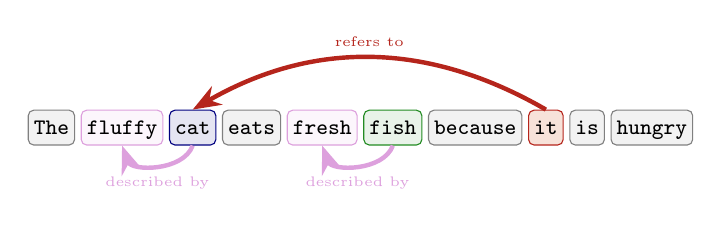
\begin{tikzpicture}
    \sentnodes{qb}
    \draw[-{Stealth}, adjcolor, line width=1.6pt] (qb2.south) to[bend left=70] node[below, font=\tiny, text=adjcolor] {described by} (qb1.south);
    \draw[-{Stealth}, adjcolor, line width=1.6pt] (qb5.south) to[bend left=70] node[below, font=\tiny, text=adjcolor] {described by} (qb4.south);
    \only<3->{
      \draw[-{Stealth}, itcolor, line width=1.6pt] (qb7.north) to[bend right=30] node[above, font=\tiny, text=itcolor] {refers to} (qb2.north);
    }
  \end{tikzpicture}
  \vfill
  \centering
  \footnotesize
  \begin{tabular}{ll}
    \toprule
    The query asks & Example \\
    \midrule
    \uncover<2->{``Adj.?''} & \uncover<2->{\tok[catcolor]{cat} $\to$ \tok[adjcolor]{fluffy} \quad \tok[fishcolor]{fish} $\to$ \tok[adjcolor]{fresh}} \\
    \uncover<3->{``Noun?''} & \uncover<3->{\tok[itcolor]{it} $\to$ \tok[catcolor]{cat}} \\
    \bottomrule
  \end{tabular}
  \normalsize
  \vfill
  \raggedright
  \begin{enumerate}
      \setcounter{enumi}{1}
    \item<4-> Same machinery - only the learned $\WQ, \WK$ differ
    \item<4-> The value of \textcolor{adjcolor}{\texttt{fluffy}} is added into \textcolor{catcolor}{\texttt{cat}}'s vector
  \end{enumerate}
  \uncover<4->{
    \small
    \[
      x_{\texttt{cat}} + \underbrace{0.55\, \vv_{\texttt{fluffy}} + 0.35\, \vv_{\texttt{cat}} + 0.10\, \vv_{\texttt{The}}}_{\text{attention output at } \texttt{cat}} \approx \text{``fluffy cat''}
    \]
    \centering
    {\scriptsize Illustrative weights - the $+$ in front is the residual connection, coming later}
  }
  \vfill
\end{frame}

\begin{frame}
  \frametitle{Scaled Dot-Product Attention}
  \vfill
  \[
    \mathrm{Attention}(\mQ, \mK, \mV) = \mathrm{softmax}\left(\frac{\mQ \mK\tr}{\sqrt{d_k}}\right) \mV
  \]
  \vfill
  % W^Q (512, 64) --x--> Q (10, 64), and the same for K and V (one head)
  \centering
  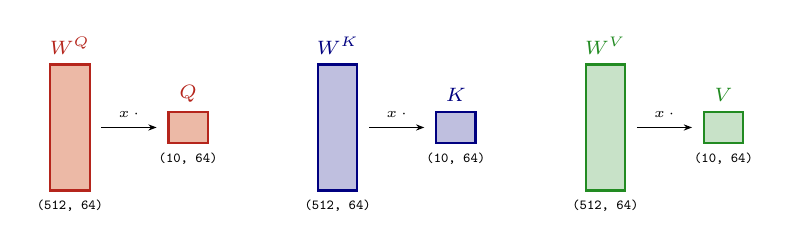
\begin{tikzpicture}[font=\scriptsize, >={Stealth[length=3pt]}]
    \foreach \c/\w/\m [count=\n from 0] in {qcolor/\WQ/\mQ, kcolor/\WK/\mK, vcolor/\WV/\mV} {
      \begin{scope}[xshift=\n*3.4cm]
        \filldraw[fill=\c!25, draw=\c, thick] (0, 0) rectangle (0.5, 1.6);
        \node[above] at (0.25, 1.6) {$\w$};
        \node[below, font=\tiny] at (0.25, 0) {\shape{512, 64}};
        \draw[->] (0.65, 0.8) -- node[above, font=\tiny] {$x\,\cdot$} (1.35, 0.8);
        \filldraw[fill=\c!25, draw=\c, thick] (1.5, 0.6) rectangle (2.0, 1.0);
        \node[above] at (1.75, 1.0) {$\m$};
        \node[below, font=\tiny] at (1.75, 0.6) {\shape{10, 64}};
      \end{scope}
    }
  \end{tikzpicture}
  \raggedright
  \only<1-3>{
    \begin{enumerate}
      \item $x_i \in \Real^{512}$ asks $\vq_i = x_i \WQ$, offers $\vk_i = x_i \WK$, and transmits $\vv_i = x_i \WV$
      \item<2-> What does $\vq_i \cdot \vk_j$ mean?
      \item<3-> Softmax produces a probability dist. called a 'score'
    \end{enumerate}
  }
  \vfill
  \only<3->{
    \begin{enumerate}
      \item<4-> What are the inputs? - $\mQ$, $\mK$, $\mV$, each \shape{10, 64}
      \item<4-> What are the outputs? - ``Update vector'' per token.
    \end{enumerate}
  }
  \vfill
\end{frame}

\begin{frame}[fragile]
  \frametitle{The Code: \texttt{attention}}
  % transformer.py L274-282
  \vfill
  \begin{lstlisting}[basicstyle=\ttfamily\tiny, xleftmargin=-0.6cm, xrightmargin=-0.6cm]
  def attention(self, Q:torch.Tensor, K:torch.Tensor, V:torch.Tensor, mask = None, dropout = None):
      d_k = Q.size(-1)
      scores = torch.matmul(Q, K.transpose(-2, -1)) / math.sqrt(d_k)
      if mask is not None:
          scores = scores.masked_fill(mask == 0, -1e9)
      p_attn = F.softmax(scores, dim = -1)
      if dropout is not None:
          p_attn = dropout(p_attn)
      return torch.matmul(p_attn, V), p_attn
  \end{lstlisting}
  \vfill
\end{frame}

\begin{frame}
  \frametitle{Why Divide by $\sqrt{d_k}$?}
  \vfill
  \begin{enumerate}
    \item<2-> $\vq$ and $\vk$ are independent with mean 0 and variance 1
    \item<3-> $\vq \cdot \vk = \sum_{i=1}^{d_k} \mathcolor{qcolor}{q_i} \mathcolor{kcolor}{k_i} \sim \mathcal{N}(\mu=0, \sigma=8)$
    \item<4-> A saturated softmax is almost one-hot - grad vanishes - the model learns slowly
      \begin{itemize}
        \item $\mathrm{softmax}(1, 2, 3) = (0.09, 0.24, 0.67)$
        \item $\mathrm{softmax}(8, 16, 24) \approx (0.00, 0.00, 1.00)$
      \end{itemize}
    \item<5-> Divide by $\sqrt{d_k} = 8$ - the scores have variance 1 again
  \end{enumerate}
  \vfill
\end{frame}

\begin{frame}
  \frametitle{Many Questions at Once}
  \vfill
  \centering
  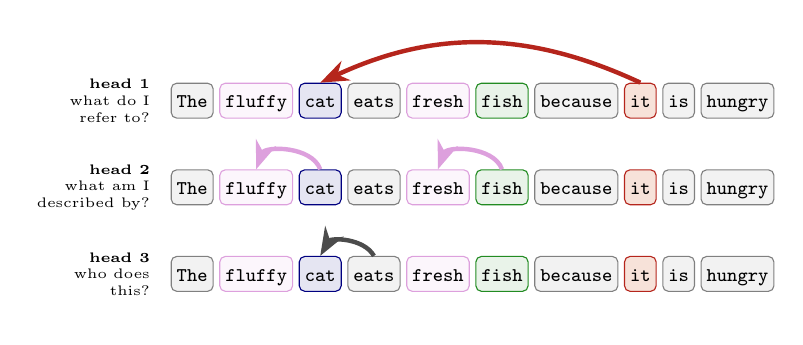
\begin{tikzpicture}[atok/.append style={font=\ttfamily\scriptsize}, mqlab/.style={font=\tiny, align=right, anchor=east, xshift=-4pt}]
    \sentnodes{ha}
    \node[mqlab] at (ha0.west) {\textbf{head 1}\\what do I\\refer to?};
    \draw[-{Stealth}, itcolor, line width=1.6pt] (ha7.north) to[bend right=25] (ha2.north);
    \begin{scope}[yshift=-1.1cm]
      \sentnodes{hb}
      \node[mqlab] at (hb0.west) {\textbf{head 2}\\what am I\\described by?};
      \draw[-{Stealth}, adjcolor, line width=1.6pt] (hb2.north) to[bend right=70] (hb1.north);
      \draw[-{Stealth}, adjcolor, line width=1.6pt] (hb5.north) to[bend right=70] (hb4.north);
    \end{scope}
    \begin{scope}[yshift=-2.2cm]
      \sentnodes{hc}
      \node[mqlab] at (hc0.west) {\textbf{head 3}\\who does\\this?};
      \draw[-{Stealth}, black!70, line width=1.6pt] (hc3.north) to[bend right=60] (hc2.north);
    \end{scope}
    \node[font=\scriptsize, gray, anchor=north east] at ([yshift=-2pt]hc9.south east) {};
  \end{tikzpicture}
  \vfill
  \raggedright
  \begin{enumerate}
    \item<2-> $h = 3$ heads, each with its own $\WQ_j, \WK_j, \WV_j \in \Real^{512 \times 64}$
    \item<3-> The 3 ``update mats'' are sent to FC Layer $W^O \in \Real^{512 \times 512}$ then a Residual Connection
  \end{enumerate}
  \vfill
\end{frame}

\begin{frame}[fragile]
  \frametitle{The Code: \texttt{MultiHeadedAttention}}
  % transformer.py L256-272 self attn
\begin{lstlisting}[basicstyle=\ttfamily\tiny, aboveskip=2pt, belowskip=2pt]
class MultiHeadedAttention(nn.Module):
  def __init__(self, h:int, d_model:int, dropout:float=0.1):
      ...
      self.d_k = d_model // h
      self.h = h
      # every head j gets its own W_q[j], W_k[j], W_v[j]: 512 -> 64
      self.W_q = nn.ModuleList([nn.Linear(d_model, self.d_k) for _ in range(h)])
      self.W_k = nn.ModuleList([nn.Linear(d_model, self.d_k) for _ in range(h)])
      self.W_v = nn.ModuleList([nn.Linear(d_model, self.d_k) for _ in range(h)])
      self.W_o = nn.Linear(d_model, d_model)
      ...
  def forward(self, x, mask=None):
      heads = []
      for j in range(self.h):
          Q, K, V = self.W_q[j](x), self.W_k[j](x), self.W_v[j](x)  # (1, 10, 64) each
          out_j, _ = self.attention(Q, K, V, mask=mask, dropout=self.dropout)  # (1, 10, 64)
          heads.append(out_j)
      return self.W_o(torch.cat(heads, dim=-1))  # 8 x (1, 10, 64) -> (1, 10, 512)
\end{lstlisting}
  \vfill
  \begin{enumerate}
    \item<2-> What are the inputs? - \texttt{x} \shape{1, 10, 512} - $\mQ$, $\mK$, $\mV$ all come from the same \texttt{x} (\emph{self}-attention)
    \item<3-> What are the outputs? - \shape{1, 10, 512} - the ``update vector'' for each token
    \item<4-> Each head $j$ has its own $\WQ_j, \WK_j, \WV_j \in \Real^{512 \times 64}$, plus one shared $W^O \in \Real^{512 \times 512}$
  \end{enumerate}
  \vfill
\end{frame}

% ---------------------------------------------------------------------------
% S4 frame: the causal mask (sentence view)
% ---------------------------------------------------------------------------
\begin{frame}[fragile]
  \frametitle{No Peeking - \texttt{subsequent\_mask}}
  % transformer.py L298, L304-306
\begin{lstlisting}[basicstyle=\ttfamily\tiny, aboveskip=2pt, belowskip=2pt]
def subsequent_mask(size):
    attn_shape = (1, size, size)
    subsequent_mask = np.triu(np.ones(attn_shape), k=1).astype('uint8')
    return torch.from_numpy(subsequent_mask) == 0
\end{lstlisting}
  % transformer.py L277-279
\begin{lstlisting}[basicstyle=\ttfamily\tiny, aboveskip=2pt, belowskip=2pt]
if mask is not None:
    scores = scores.masked_fill(mask == 0, -1e9)
p_attn = F.softmax(scores, dim = -1)
\end{lstlisting}
  \begin{columns}[T]
    \begin{column}{0.31\textwidth}
      \centering
      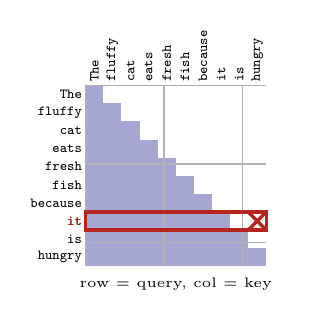
\begin{tikzpicture}[x=0.23cm, y=-0.23cm, font=\tiny\ttfamily]
        \foreach \r in {0,...,9} {
          \foreach \c in {0,...,\r} {
            \fill[catcolor!35] (\c, \r) rectangle ++(1, 1);
          }
        }
        \draw[gray!60] (0, 0) grid (10, 10);
        \foreach \w [count=\i from 0] in {The,fluffy,cat,eats,fresh,fish,because,it,is,hungry} {
          \node[anchor=east, inner sep=1pt] at (0, \i+0.5) {\w};
          \node[anchor=west, inner sep=1pt, rotate=90] at (\i+0.5, 0) {\w};
        }
        \node[anchor=east, inner sep=1pt, text=itcolor] at (0, 7.5) {it};
        \only<2->{
          \draw[itcolor, very thick] (0, 7) rectangle (10, 8);
          \draw[itcolor, very thick] (9, 7) -- (10, 8) (9, 8) -- (10, 7);
        }
        \node[font=\tiny, anchor=north] at (5, 10.1) {row = query, col = key};
      \end{tikzpicture}
    \end{column}
    \begin{column}{0.67\textwidth}
      \setbeamerfont{itemize/enumerate body}{size=\footnotesize}
      \begin{enumerate}
        \item<2-> Row \textcolor{itcolor}{\texttt{it}} cannot see \texttt{is}, \texttt{hungry} - when we write, they do not exist yet
      \end{enumerate}
    \end{column}
  \end{columns}
  \vfill
\end{frame}

\againframe<4>{decarch}

\section*{Block}

% ---------------------------------------------------------------------------
% S5 frame: feed-forward
% ---------------------------------------------------------------------------
\begin{frame}[fragile]
  \frametitle{What Do We Know About Cats?}
  \smallskip
  % transformer.py L31, L38-44, L49
  {\small Cats get hungry, fish get eaten - none of that is \emph{in} the sentence\par}
  \vfill
  \begin{lstlisting}[basicstyle=\ttfamily\tiny]
  class PositionwiseFeedForward(nn.Module):
      def __init__(self, d_model: int, d_ff: int, dropout:float=0.1):
          super(PositionwiseFeedForward, self).__init__()
          self.w1 = nn.Linear(d_model, d_ff)
          self.w2 = nn.Linear(d_ff, d_model)
          self.dropout = nn.Dropout(dropout)
      def forward(self, x:torch.Tensor):
          return self.w2(self.dropout(F.selu(self.w1(x))))
  \end{lstlisting}
  \vfill
  {\small Attention mixes \emph{across} tokens, the FFN works \emph{within} a token; ``position-wise'' = per position - it adds no position information}
\end{frame}

% ---------------------------------------------------------------------------
% S5 frame: residuals and LayerNorm
% ---------------------------------------------------------------------------
\begin{frame}[fragile]
  \frametitle{Numerical Stability: Residuals and LayerNorm}
  \centering
  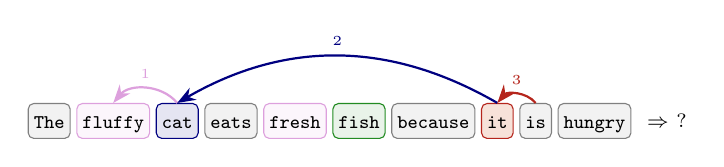
\begin{tikzpicture}[atok/.append style={font=\ttfamily\scriptsize}]
    \sentnodes{rs}
    \path (rs0.north) ++(0, 0.9);
    \draw[-{Stealth}, adjcolor, thick] (rs2.north) to[bend right=50] node[above, font=\tiny] {1} (rs1.north);
    \draw[-{Stealth}, catcolor, thick] (rs7.north) to[bend right=30] node[above, font=\tiny] {2} (rs2.north);
    \draw[-{Stealth}, itcolor, thick] (rs8.north) to[bend right=50] node[above, font=\tiny] {3} (rs7.north);
    \node[font=\scriptsize, anchor=west] at ($(rs9.east)+(2pt, 0)$) {$\Rightarrow$ ?};
  \end{tikzpicture}
  \par
  {\scriptsize \texttt{cat} $\leftarrow$ \texttt{fluffy}, then \texttt{it} $\leftarrow$ \texttt{cat}, then \texttt{is} $\leftarrow$ \texttt{it}, plus ``cats get hungry'' - several rounds $\Rightarrow$ stack $N = 6$ blocks\par}
  \vfill
  % transformer.py L26-28 (LayerNorm.forward)
  \begin{lstlisting}[basicstyle=\ttfamily\tiny]
  class LayerNorm(nn.Module):
      def forward(self, x):
          mean = x.mean(-1, keepdim=True)
          std = x.std(-1, keepdim=True)
          return self.alpha * ((x - mean) / (std + self.eps)) + self.bias
  \end{lstlisting}
  % transformer.py L130 (SubLayerConnection.forward), written out for the two things it wraps: self_attn, then feed_forward
  \begin{lstlisting}[basicstyle=\ttfamily\tiny]
  class EncoderLayer(nn.Module):
      def forward(self, x, mask):
          x = x + self.dropout(self.self_attn(self.norm1(x), mask))  # attention
          return x + self.dropout(self.feed_forward(self.norm2(x)))  # feed-forward
  \end{lstlisting}
\end{frame}

% ---------------------------------------------------------------------------
% S5 frame: key moment 2 - EncoderLayer + causal mask is a GPT block
% ---------------------------------------------------------------------------
\begin{frame}[fragile]
  \frametitle{GPT2 - 2019}
  % transformer.py L143, L147-148 (EncoderLayer.forward), self_attn(y, y, y, mask) -> self_attn(y, mask) to match the simplified MultiHeadedAttention
  % the two self.sublayer[i](x, f) wrapper calls are written out as x + dropout(f(norm_i(x)))
  \vfill
  \begin{lstlisting}[basicstyle=\ttfamily\tiny]
  class EncoderLayer(nn.Module):
      def __init__(self, size, self_attn, feed_forward, dropout):
          ...
          self.norm1, self.norm2 = LayerNorm(size), LayerNorm(size)
      def forward(self, x, mask):
          x = x + self.dropout(self.self_attn(self.norm1(x), mask))
          return x + self.dropout(self.feed_forward(self.norm2(x)))
  \end{lstlisting}
  % transformer.py L156-157, L159-163 (Encoder)
  \begin{lstlisting}[basicstyle=\ttfamily\tiny]
  class Encoder(nn.Module):
      def __init__(self, layer, N):
          ...
          self.layers = nn.ModuleList([copy.deepcopy(layer) for _ in range(N)])
          self.norm = LayerNorm(layer.size)
      def forward(self, x, mask):
          for layer in self.layers:
              x = layer(x, mask)
          return self.norm(x)
  \end{lstlisting}
  \vfill
  \setbeamerfont{itemize/enumerate body}{size=\footnotesize}
  \begin{enumerate}
    \item<2-> What are the inputs? - \texttt{x} \shape{1, 10, 512}, \texttt{mask} \shape{1, 10, 10}
    \item<2-> What are the outputs? - \shape{1, 10, 512} - the enhanced representation of each token, after $N$ rounds
  \end{enumerate}
  \vfill
\end{frame}

\againframe<5>{decarch}

% ---------------------------------------------------------------------------
% S5 frame: generator (model-input view)
% ---------------------------------------------------------------------------
\begin{frame}[fragile]
  \frametitle{Choosing the Next Word - \texttt{Generator}}
  \begin{columns}[c]
    \begin{column}{0.56\textwidth}
      % transformer.py L51, L55-57, L59, L69
\begin{lstlisting}[basicstyle=\ttfamily\tiny]
class Generator(nn.Module):
    def __init__(self, d_model, vocab):
        super(Generator, self).__init__()
        self.proj = nn.Linear(d_model, vocab)
    def forward(self, x):
        return F.log_softmax(self.proj(x), dim=-1)
\end{lstlisting}
    \end{column}
    \begin{column}{0.42\textwidth}
      \centering
      \uncover<3->{%
        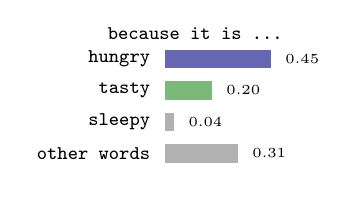
\begin{tikzpicture}[font=\scriptsize, x=3.0cm, y=0.4cm]
          \node[anchor=south, font=\scriptsize, inner sep=0pt] at (0.15, 0.6) {\texttt{because it is \dots\ }};
          \foreach \w/\p/\c [count=\i from 0] in {hungry/0.45/catcolor, tasty/0.20/fishcolor, sleepy/0.04/gray, other words/0.31/gray} {
            \node[anchor=east, font=\ttfamily\scriptsize] at (0, -\i) {\w};
            \fill[\c!60] (0.02, -\i-0.3) rectangle (0.02+\p, -\i+0.3);
            \node[anchor=west, font=\tiny] at (0.04+\p, -\i) {\p};
          }
        \end{tikzpicture}\par
      }
    \end{column}
  \end{columns}
  \vfill
  \setbeamerfont{itemize/enumerate body}{size=\footnotesize}
  \begin{enumerate}
    \item<2-> What are the inputs? - enhanced token representations \shape{1, 10, 512}
    \item<3-> What are the outputs? - \shape{1, 10, V} - log-probs for the word after position $t$
  \end{enumerate}
\end{frame}

% ---------------------------------------------------------------------------
\begin{frame}[fragile]
  \frametitle{Our GPT2 - 2019}
  % assembled from transformer.py classes; tested in decoder_only/assembly_snippet.py
\begin{lstlisting}[basicstyle=\ttfamily\tiny,xleftmargin=-8pt,xrightmargin=-8pt]
class DecoderOnlyLM(nn.Module):
    def __init__(self, V, N=6, d_model=512, d_ff=1024, h=8, dropout=0.1):
        super().__init__()
        c = copy.deepcopy
        attn, ff = MultiHeadedAttention(h, d_model), PositionwiseFeedForward(d_model, d_ff, dropout)
        self.embed = nn.Sequential(Embeddings(d_model, V), PositionalEncoding(d_model, dropout))
        self.blocks = Encoder(EncoderLayer(d_model, c(attn), c(ff), dropout), N)
        self.generator = Generator(d_model, V)
        [nn.init.xavier_uniform_(p) for p in self.parameters() if p.dim() > 1]
    def forward(self, x):                            # x: (batch, n) token ids
        mask = Batch.subsequent_mask(x.size(1))      # (1, n, n), True on/below diagonal
        return self.generator(self.blocks(self.embed(x), mask))   # (batch, n, V) log-probs
\end{lstlisting}
  \vfill
  \footnotesize
  \begin{enumerate}
    \item<2-> What are the inputs? - ids of \texttt{<s> The \dots\ it is}
      \shape{1, 10}
    \item<3-> What are the outputs? - next word log-probs \shape{1, 10, V}
    \item<4-> Called a ``decoder-only'' model because it performs the decoding step
  \end{enumerate}
  \vfill
\end{frame}

\againframe<6>{decarch}

% ---------------------------------------------------------------------------
% S4 frame: the next-token task (model-input view)
% ---------------------------------------------------------------------------
\begin{frame}[fragile]
  \frametitle{The Task: Predict the Next Word}
  \centering
  {\scriptsize
    \setlength{\tabcolsep}{2.5pt}
    \begin{tabular}{r|cccccccccc}
      $t$ & 0 & 1 & 2 & 3 & 4 & 5 & 6 & 7 & 8 & 9 \\
      \hline
      \texttt{trg} & \texttt{<s>} & \texttt{The} & \texttt{\textcolor{adjcolor}{fluffy}} &
      \texttt{\textcolor{catcolor}{cat}} & \texttt{eats} & \texttt{\textcolor{adjcolor}{fresh}} &
      \texttt{\textcolor{fishcolor}{fish}} & \texttt{because} & \texttt{\textcolor{itcolor}{it}} &
      \alt<2->{\textbf{\texttt{is}}}{\texttt{is}} \\
      \texttt{trg\_y} & \texttt{The} & \texttt{\textcolor{adjcolor}{fluffy}} &
      \texttt{\textcolor{catcolor}{cat}} & \texttt{eats} & \texttt{\textcolor{adjcolor}{fresh}} &
      \texttt{\textcolor{fishcolor}{fish}} & \texttt{because} & \texttt{\textcolor{itcolor}{it}} &
      \texttt{is} & \alt<2->{\textbf{\texttt{hungry}}}{\texttt{hungry}} \\
    \end{tabular}
  }
  \par
  \raggedright
  \vfill
  \setbeamerfont{itemize/enumerate body}{size=\footnotesize}
  \begin{enumerate}
    \item<2-> loss function = cross-entropy between soft target \texttt{trg\_y} and the log-probs from \texttt{Generator}
  \end{enumerate}
\end{frame}

% ---------------------------------------------------------------------------
\begin{frame}[fragile]
  \frametitle{Generating Text - One Word at a Time}
  \centering
  {\scriptsize
    \begin{tabular}{r@{\quad$\to$\quad}l}
      \tok{<s>} & \tok{The} \\
      \tok{<s>} \tok{The} & \tok[adjcolor]{fluffy} \\
      \tok{<s>} \tok{The} \tok[adjcolor]{fluffy} & \tok[catcolor]{cat} \\
      $\vdots$ & $\vdots$ \\
      \tok{<s>} \tok{The} \dots\ \tok{because} \tok[itcolor]{it} & \tok{is} \\
      \tok{<s>} \tok{The} \dots\ \tok[itcolor]{it} \tok{is} &
      \tok{hungry} \,/\, \tok{tasty} \\
    \end{tabular}
  }
  \vfill
\end{frame}

\section*{Transformer}

\begin{frame}
  \frametitle{Ok Then What is A Transformer?}
  \begin{enumerate}
    \item Imagine you wanted to translate between English and German
    \item<2-> The \emph{encoder} reads the English (\texttt{src}), the \emph{decoder} writes the German (\texttt{trg}) one word at a time
  \end{enumerate}
  \vfill
  \centering
  \visible<2->{%
    \makebox[\textwidth][c]{%
      \begin{tikzpicture}[
          >={Stealth[length=3pt]},
          atok/.append style={font=\ttfamily\tiny},
          fulllab/.style={font=\scriptsize, inner sep=1pt},
        ]
        % src (top): the English sentence, read by the encoder
        \sentnodes{en}
        % trg (below): the German translation, written by the decoder,
        % lined up on the fresh|fish boundary so the cross-attention lines stay short
        \node[atok=adjcolor, anchor=east] (de4) at ($(en4.east)!0.5!(en5.west) + (-1pt, -1.7cm)$) {frischen};
        \node[atok, left=2pt of de4] (de3) {frisst};
        \node[atok=catcolor, left=2pt of de3] (de2) {Katze};
        \node[atok=adjcolor, left=2pt of de2] (de1) {flauschige};
        \node[atok, left=2pt of de1] (de0) {Die};
        \node[atok=fishcolor, right=2pt of de4] (de5) {Fisch};
        \node[atok, right=2pt of de5] (de6) {weil};
        \node[atok=itcolor, right=2pt of de6] (de7) {sie};
        \node[atok, right=2pt of de7] (de8) {hungrig};
        \node[atok, right=2pt of de8] (de9) {ist};
        \node[fulllab, anchor=east] at ([xshift=-4pt]en0.west) {\texttt{src}};
        \node[fulllab, anchor=east] at ([xshift=-4pt]de0.west) {\texttt{trg}};
        % reserve the space of the encoder arcs above src on every overlay
        \path (en0.north) ++(0, 1.15);
        % <3> encoder self-attention: no mask, it looks both ways, even at hungry
        \only<3->{
          \foreach \j in {0, ..., 6}
          \draw[->, black!40] (en7.north) to[out=110, in=70, looseness=0.5] (en\j.north);
          \foreach \j in {8, 9}
          \draw[->, black!40] (en7.north) to[out=70, in=110, looseness=0.9] (en\j.north);
          \node[fulllab, text=black!70, anchor=south] at ($(en0.north)!0.5!(en9.north) + (0, 0.85)$)
          {encoder: no mask};
        }
        % <4> cross-attention: each German word asks the English sentence
        % (illustrative alignment; hungrig/ist cross because German puts the verb last)
        \only<4->{
          \foreach \d/\e in {0/0, 1/1, 2/2, 3/3, 4/4, 5/5, 6/6}
          \draw[->, black!35] (de\d.north) -- (en\e.south);
          \draw[->, black!75, thick] (de8.north) -- (en9.south);
          \draw[->, black!75, thick] (de9.north) -- (en8.south);
          \draw[->, itcolor, very thick] (de7.north) -- (en7.south);
        }
        % <5> sie (not er): the decoder needs it = cat
        \only<5->{
          \draw[->, catcolor, thick, dashed] (de7.north) -- (en2.south);
        }
      \end{tikzpicture}%
    }%
  }
  \vfill
  \raggedright
  \begin{enumerate}
      \setcounter{enumi}{2}
    \item<3-> The English is all there - drop the causal mask: the
      \emph{encoder} is our \texttt{EncoderLayer} with only a padding
      \texttt{src\_mask} \shape{1, 1, m}
    \item<4-> The decoder still writes left to right, and asks questions
      \emph{of the English} - \emph{cross-attention}
      {\scriptsize (weights illustrative)}
    \item<5-> \textcolor{itcolor}{\texttt{sie}}, not \texttt{er} - \emph{die} Katze but \emph{der} Fisch, so the decoder needs \textcolor{itcolor}{\texttt{it}} = \textcolor{catcolor}{\texttt{cat}}; and \texttt{ist} comes last - the lines cross
  \end{enumerate}
\end{frame}

\begin{frame}
  \frametitle{The 2017 Transformer%
  \only<2>{ - Encoder}\only<3>{ - Decoder}\only<4>{ - Memory}}
  \centering
  \makebox[\textwidth][c]{%
    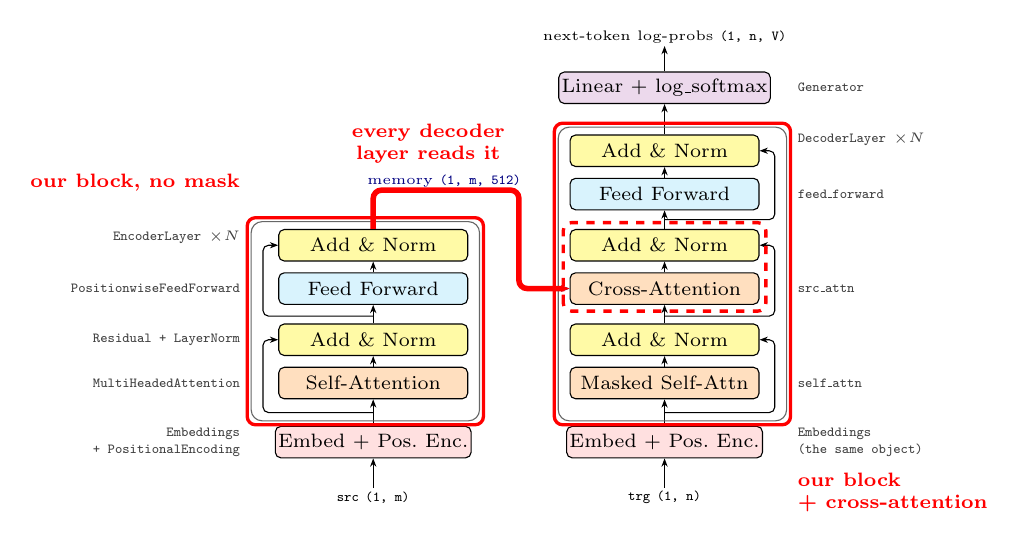
\begin{tikzpicture}[
        x=1cm, y=1cm, font=\scriptsize,
        >={Stealth[length=3pt]},
        fblk/.style={draw, rounded corners=2pt, minimum width=2.4cm,
        minimum height=0.4cm, inner sep=1pt},
        fattn/.style={fblk, fill=orange!25},
        fffn/.style={fblk, fill=cyan!15},
        fnorm/.style={fblk, fill=yellow!35},
        femb/.style={fblk, fill=red!12},
        fgen/.style={fblk, fill=violet!15},
        fcls/.style={font=\tiny\ttfamily, text=black!75, inner sep=1pt},
        fio/.style={font=\tiny, inner sep=1pt},
        fhl/.style={draw=Red, very thick, rounded corners=3pt},
        fnote/.style={font=\scriptsize\bfseries, text=Red, inner sep=1pt},
      ]
      % ---------- encoder (x = 0) ----------
      \node[fio] (fein) at (0, 0) {\texttt{src} \shape{1, m}};
      \node[femb] (feemb) at (0, 0.7) {Embed + Pos.\ Enc.};
      \node[fattn] (featt) at (0, 1.45) {Self-Attention};
      \node[fnorm] (fen1) at (0, 2.0) {Add \& Norm};
      \node[fffn] (feff) at (0, 2.65) {Feed Forward};
      \node[fnorm] (fen2) at (0, 3.2) {Add \& Norm};
      \foreach \a/\b in {fein/feemb, feemb/featt, featt/fen1, fen1/feff, feff/fen2}
      \draw[->] (\a) -- (\b);
      % residuals (left side)
      \draw[->, rounded corners=2pt] (0, 1.075) -| (-1.4, 2.0) -- (fen1.west);
      \draw[->, rounded corners=2pt] (0, 2.3) -| (-1.4, 2.65) |- (fen2.west);
      \draw[rounded corners=4pt, black!60] (-1.55, 0.97) rectangle (1.35, 3.5);
      % ---------- decoder (x = 3.7) ----------
      \node[fio] (fdin) at (3.7, 0) {\texttt{trg} \shape{1, n}};
      \node[femb] (fdemb) at (3.7, 0.7) {Embed + Pos.\ Enc.};
      \node[fattn] (fdatt) at (3.7, 1.45) {Masked Self-Attn};
      \node[fnorm] (fdn1) at (3.7, 2.0) {Add \& Norm};
      \node[fattn] (fdsrc) at (3.7, 2.65) {Cross-Attention};
      \node[fnorm] (fdn2) at (3.7, 3.2) {Add \& Norm};
      \node[fffn] (fdff) at (3.7, 3.85) {Feed Forward};
      \node[fnorm] (fdn3) at (3.7, 4.4) {Add \& Norm};
      \node[fgen] (fgen) at (3.7, 5.2) {Linear + log\_softmax};
      \node[fio] (fdout) at (3.7, 5.85) {next-token log-probs \shape{1, n, V}};
      \foreach \a/\b in {fdin/fdemb, fdemb/fdatt, fdatt/fdn1, fdn1/fdsrc, fdsrc/fdn2,
      fdn2/fdff, fdff/fdn3, fdn3/fgen, fgen/fdout}
      \draw[->] (\a) -- (\b);
      % residuals (right side)
      \draw[->, rounded corners=2pt] (3.7, 1.075) -| (5.1, 2.0) -- (fdn1.east);
      \draw[->, rounded corners=2pt] (3.7, 2.3) -| (5.1, 2.65) |- (fdn2.east);
      \draw[->, rounded corners=2pt] (3.7, 3.525) -| (5.1, 3.85) |- (fdn3.east);
      \draw[rounded corners=4pt, black!60] (2.35, 0.97) rectangle (5.25, 4.7);
      % ---------- memory: encoder output -> cross-attention ----------
      \draw[->, very thick, catcolor, rounded corners=3pt]
      (fen2.north) -- (0, 3.9) -| (1.85, 2.65) -- (fdsrc.west);
      \node[fio, anchor=south, text=catcolor] at (0.9, 3.9)
      {memory \shape{1, m, 512}};
      % ---------- class names (left: encoder) ----------
      \node[fcls, anchor=east, align=right] at (-1.65, 0.7)
      {Embeddings\\+ PositionalEncoding};
      \node[fcls, anchor=east] at (-1.65, 1.45) {MultiHeadedAttention};
      \node[fcls, anchor=east] at (-1.65, 2.0) {Residual + LayerNorm};
      \node[fcls, anchor=east] at (-1.65, 2.65) {PositionwiseFeedForward};
      \node[fcls, anchor=east] at (-1.65, 3.3) {\textbf{EncoderLayer} $\times N$};
      % ---------- attribute / class names (right: decoder) ----------
      \node[fcls, anchor=west, align=left] at (5.35, 0.7)
      {Embeddings\\(the same object)};
      \node[fcls, anchor=west] at (5.35, 1.45) {self\_attn};
      \node[fcls, anchor=west] at (5.35, 2.65) {src\_attn};
      \node[fcls, anchor=west] at (5.35, 3.85) {feed\_forward};
      \node[fcls, anchor=west] at (5.35, 4.55) {\textbf{DecoderLayer} $\times N$};
      \node[fcls, anchor=west] at (5.35, 5.2) {Generator};
      % ---------- highlights ----------
      \draw<2>[fhl] (-1.6, 0.92) rectangle (1.4, 3.55);
      \node<2>[fnote, anchor=east] at (-1.65, 4.0) {our block, no mask};
      \draw<3>[fhl] (2.3, 0.92) rectangle (5.3, 4.75);
      \draw<3>[fhl, dashed] ($(fdsrc.south west) + (-0.08, -0.08)$)
      rectangle ($(fdn2.north east) + (0.08, 0.08)$);
      \node<3>[fnote, anchor=north west, align=left] at (5.35, 0.35)
      {our block\\+ cross-attention};
      \draw<4>[->, line width=2pt, Red, rounded corners=3pt]
      (fen2.north) -- (0, 3.9) -| (1.85, 2.65) -- (fdsrc.west);
      \node<4>[fnote, anchor=south, align=center] at (0.7, 4.2)
      {every decoder\\layer reads it};
    \end{tikzpicture}%
  }

  \vfill
\end{frame}

\begin{frame}{Thank you!}
  Helpful Links
  \vfill
  \begin{enumerate}
    \item Attention Is All You Need - https://arxiv.org/abs/1706.03762
    \item The Annotated Transformer - https://nlp.seas.harvard.edu/2018/04/03/attention.html
    \item Code - https://github.com/GersiD/ML/tree/main/transformer
    \item Slides - Email me Gersi.Doko@unh.edu
  \end{enumerate}
\end{frame}

\end{document}
